\chapter{Aplicación sigue personas}
\label{cap:capitulo5}
Ahora que ya tenemos integrado ROS2 dentro de la plataforma de VisualCircuit, vamos a crear varios proyectos usando los bloques drivers que hemos creado.
El primero de ellos será un comportamiento de \textit{follow-person} usando reconocimiento visual.

\section{Desarrollo inicial sigue-personas (sólo rotación)}
\label{sec:FP_intro}

El comportamiento sigue-persona que buscamos desarrollar con VisualCircuit consiste en rotar en círculos hasta encontrar a una persona mediante
algoritmos de detección visual de objetos y mantener a la persona centrada en la imagen, al igual que mantenernos a una distancia constante,
usando así la función de lectura de distancias de la cámara. Por ello sólamente la cámara como sensor, ya que esta función mencionada nos permite no
usar el láser y evitar un código más complejo.\\

En una primera aproximación, buscaremos sólo mantener a la persona centrada usando únicamente movimiento angular y, una vez que tengamos esta parte funcionando,
añadiremos la parte del comportamiento que implica seguir a la persona también linealmente.\\

En primer lugar, debemos preparar el entorno de pruebas, por lo que aprovecharemos un modelo de persona teleoperada que creó Carlos
Caminero\footnote{\url{https://github.com/RoboticsLabURJC/2021-tfg-carlos-caminero/tree/main/amazon_hospital/hospital_world}}, compañero de la carrera.

\begin{figure} [H]
    \begin{center}
        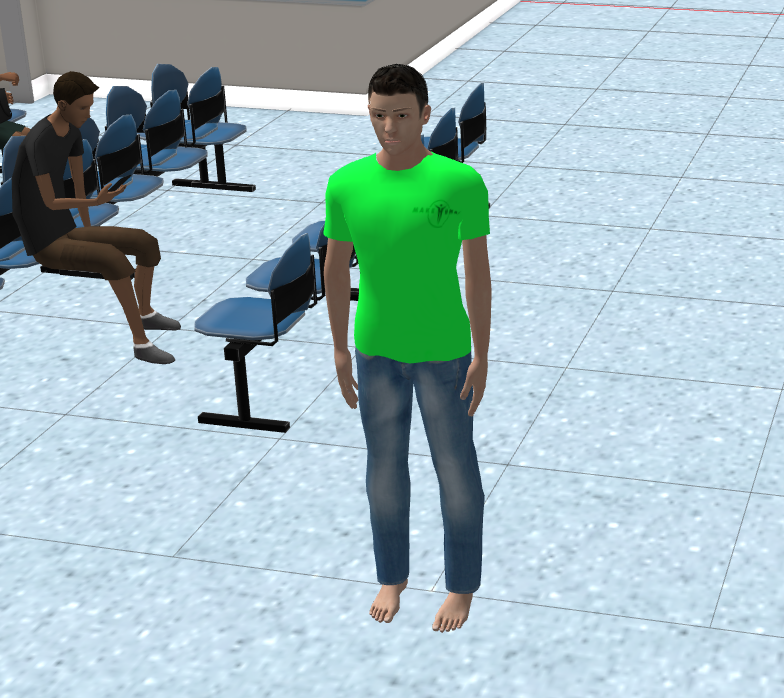
\includegraphics[width=7cm]{figs/c5/elman.png}
    \end{center}
    \caption[Modelo de persona en gazebo]{Modelo de persona teleoperable en gazebo.}
    \label{fig:teleop_person}
\end{figure}
El mundo que tenía Carlos creado incluía muchos elementos del entorno que no son necesarios en nuestro caso, por lo que modificaremos el
mundo para dejar únicamente al robot y a la persona. El modelo del robot que usaremos será el que mencionamos en el capítulo \ref{subsec:turtlebot2_sim},
ya que incluye tanto cámara como láser.\\

\begin{figure} [H]
    \begin{center}
        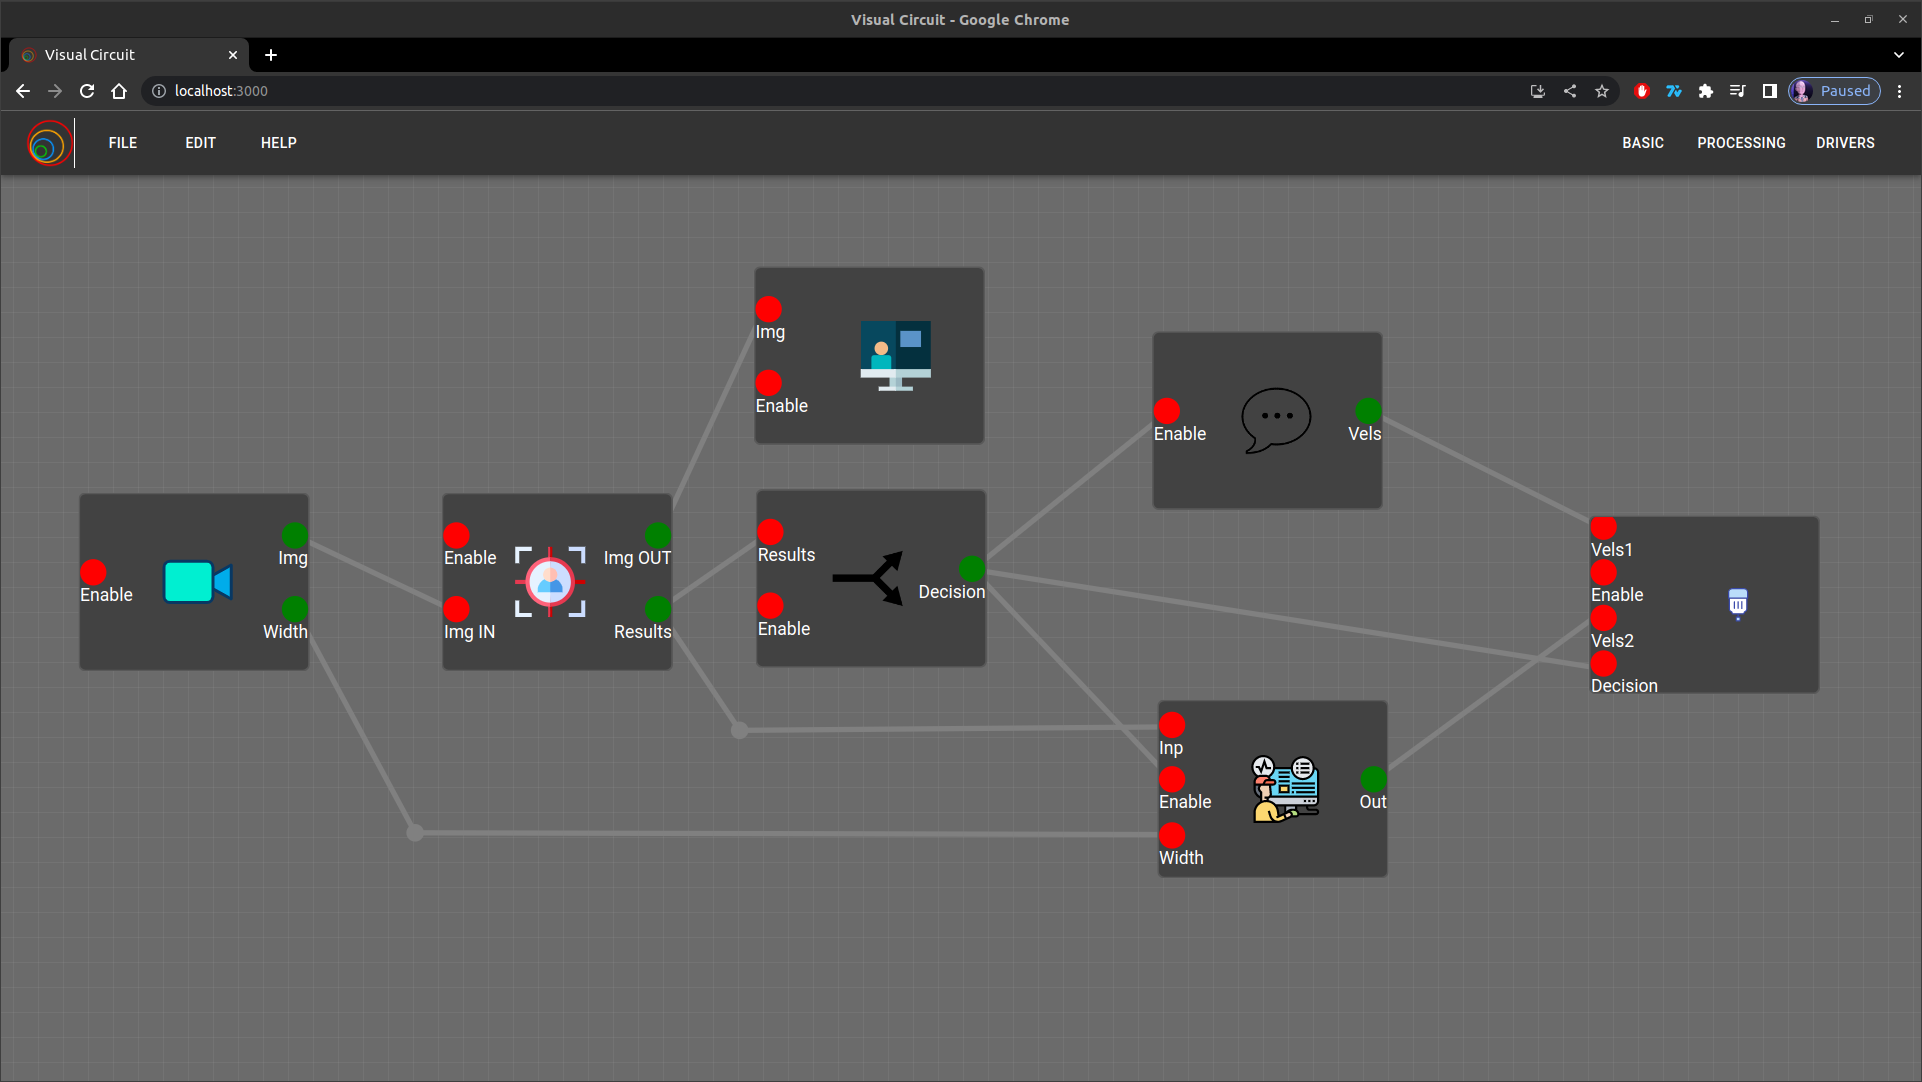
\includegraphics[width=12cm]{figs/c5/follow_person_initial.png}
    \end{center}
    \caption[Circuito sigue-personas inicial]{Circuito inicial del algoritmo sigue-persona.}
    \label{fig:initial_follow_person}
\end{figure}

La lógica que seguirá será la siguiente: recibir la imagen del \textit{topic} de la cámara y compartirla con el bloque de detección de objetos,
enviar la imagen con las detecciones al bloque \textit{screen} para visualizar en tiempo real lo que está analizando el robot,
y también mandaremos los resultados a un bloque que decidirá qué hacer. Este bloque activa un PID en caso de que haya una persona en la imagen,
o el comportamiento de rotación en caso de que no se haya encontrado ninguna.
En ambos casos, se envía la decisión a los bloques que generan las velocidades y también al bloque \textit{MotorDriver} que hemos creado en
el punto \ref{sec:drivers_creacion}, que recibe tanto las distintas velocidades, como la decisión que se ha tomado, y envía al \textit{topic} la adecuada.

La detección visual utiliza yolov3\footnote{\textbf{YouOnlyLookOnce (YOLO)}: \url{https://pjreddie.com/darknet/yolo/}},
un algoritmo de detección de objetos a tiempo real que permite identificarlos tanto en video como en imágenes usando redes neuronales
(darknet\footnote{\textbf{DarkNet}: \url{https://pjreddie.com/darknet/}}). El bloque que ya está integrado en VisualCircuit nos sirve para nuestra aplicación,
pero he tenido que modificarlo para poder extraer también la localización de la \textit{Bounding Box} que corresponde a la persona y compartirla con otros bloques.\\

Para ello, después de obtener los nombres de los objetos encontrados, recorremos toda la lista comprobando si hay alguna persona,
en caso de haberla enviamos la \textit{Bounding Box} correspondiente, sino, enviamos un \textit{array} con cuatro valores ``-1'' para indicar que está vacío.

\begin{code}[H]
    \begin{lstlisting}[language=python]
    #**********
        #forward Pass
        results = net.forward(outputNames)
        findObjects(results,frame)
        is_person = False
        for i in classIds:
            if(className[i] == "person"):
                is_person = True
                break
        to_send = [-1,-1,-1,-1]
        if(is_person):
            to__send = bbox[i]
        outputs.share_image("Img OUT", frame)
        outputs.share_array("Results", to__send)
        synchronise()
    #**********
    \end{lstlisting}
    \caption[Modificación al bloque detector de objetos]{Modificación al bloque de la detección de objetos.}
    \label{cod:mod_object_detector}
\end{code}

El siguiente bloque (\ref{cod:decision_follow_person}) es el que toma las decisiones de qué comportamiento seguir.
Para ello, primero esperaremos hasta recibir algún resultado de la visión y así no movernos antes haber podido analizar la situación.\\
Una vez que tengamos resultados, miraremos si es una \textit{Bounding Box} válida, en caso de serlo, la decisión será seguir lo que indique el bloque PID.
En caso de ser una caja vacía (\textit{array} de ``-1'') activaremos un contador para aplicar un filtro de paso bajo.\\
Este filtro nos permite evitar cambiar de comportamiento por pequeños errores en la detección de objetos.
Está establecido a 10, por lo que al llegar a 10 imágenes seguidas sin una persona en la imágen, cambiaremos de comportamiento al de la rotación.\\

\begin{code}[H]
    \begin{lstlisting}[language=python]
        def main(inputs, outputs, parameters, synchronise):
            auto_enable = True
            try:
                enable = inputs.read_number("Enable")
            except Exception:
                auto_enable = True
             
            while(True):
            # Wait for results
                results = inputs.read_array("Results")
                try:
                    if(results.any()):
                        break
                except Exception:
                    continue
    
            not_to_enable = 0
            to_enable = 1
            lowpass_filter = 10
            counter = 0
            print("EMPEZAMOS")

            while(auto_enable or inputs.read_number('Enable')):
                results = inputs.read_array("Results")
                if(results[0] != -1):
                    # Follow
                    counter = 0
                    outputs.share_number("Decision", 1)
                elif(counter < lowpass_filter):
                    # Follow but low-pass filter
                    counter += 1
                    outputs.share_number("Decision", 2)
                else:
                    # Rotation
                    outputs.share_number("Decision", 0)
    \end{lstlisting}
    \caption[Código bloque decisión sigue-persona]{Código del bloque de decisiones del sigue-persona.}
    \label{cod:decision_follow_person}
\end{code}

En cuanto al bloque que envía la velocidad correspondiente al comportamiento de rotación, tiene un bucle que lee el cable que le llega, en caso de
ser un "1" (\textit{True}) informa en la terminal que estamos rotando y envía una velocidad angular de 1rad/s para el eje Z.

\begin{code}[H]
    \begin{lstlisting}[language=python]
    import numpy as np

    def main(inputs, outputs, parameters, synchronise):
        try:
            while 1:
                if(inputs.read_number('Enable')):
                    print("ROT")
                    vels = [0,0,0,0,0,1]
                    to_write = np.array(vels, dtype='<U64')
                    outputs.share_array("Vels", to_write)   
                    synchronise()
        except Exception as e:
            print("Error")
    \end{lstlisting}
    \caption[Código bloque rotación sigue-persona]{Código del bloque de la rotación del sigue-persona.}
    \label{cod:rotation_follow_person}
\end{code}

En paralelo al anterior, también se puede activar el bloque PID\footnote{
    \textbf{PID}: Controlador proporciona, integral y derivativo.
        Mecanismo de control que, mediante sistema en lazo cerrado (realimentación), permite regular
        un valor (velocidad, temperatura, presión, etc)}.
Su estructura consiste en tres entradas (Resultados de la detección de objetos, ancho de la imagen y \textit{enable}), tres parámetros para las
tres constantes del controlador y una salida para la velocidad lineal y angular final que aplicaremos al robot.

\begin{figure} [H]
    \begin{center}
        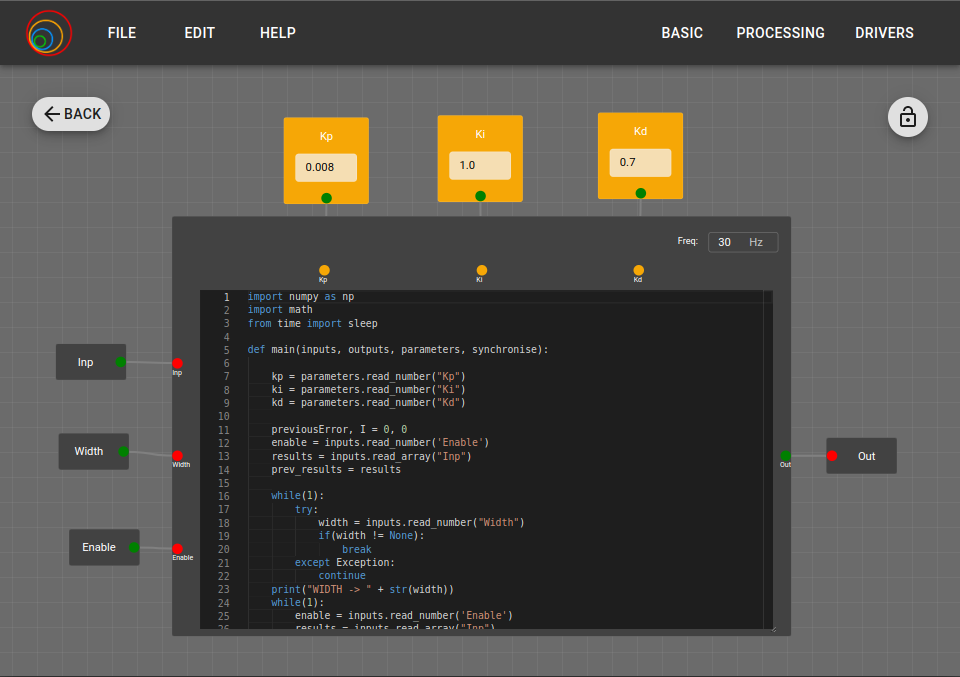
\includegraphics[width=10cm]{figs/c5/PID_follow_person.png}
    \end{center}
    \caption[Circuito del bloque PID sigue-persona]{Circuito del bloque PID del sigue-persona en VisualCircuit.}
    \label{fig:PID_follow_person}
\end{figure}

Analizando el código del bloque PID (\ref{cod:PID_follow_person}), podemos ver que primero lee los tres parámetros del controlador y entramos en el
mismo bucle que hemos mencionado en el código bloque de decisión (\ref{cod:decision_follow_person}), donde esperamos hasta obtener datos para
empezar a trabajar. Después, en el bucle principal sólo se analizan y envían los datos del PID en caso de que el bloque haya sido activado.\\

\begin{code}[H]
    \begin{lstlisting}[language=python]
        def main(inputs, outputs, parameters, synchronise):
            kp = parameters.read_number("Kp")
            ki = parameters.read_number("Ki")
            kd = parameters.read_number("Kd")
            previousError = 0
            I = 0
            max_rotation = 1
            enable = inputs.read_number('Enable')
            results = inputs.read_array("Inp")
            prev_results = results
        
            #Wait for values
            while(1):
                try:
                    width = inputs.read_number("Width")
                    if(width != None):
                        break
                except Exception:
                    continue
            while(1):
                enable = inputs.read_number('Enable')
                results = inputs.read_array("Inp")
                if(enable != 0):
                    try:        
                        if(enable == 1):
                            error = float(results[0]+results[2]/2) - width/2
                            prev_results = results
                        P = error
                        D = float(error) - float(previousError)
                        PIDvalue = (kp*P)  + (kd*D)
                        previousError = float(error)

                        angular_velocity = -PIDvalue
                        if(angular_velocity > max_rotation or angular_velocity < -max_rotation):
                            angular_velocity = max_rotation*angular_velocity/abs(angular_velocity)
                        data = [0,0,0,0,0, angular_velocity]
                        outputs.share_array("Out", data)
        
                        synchronise()
                    except Exception:
                        synchronise()
                        continue
    \end{lstlisting}
    \caption[Código bloque PID sigue-persona]{Código del bloque del PID sigue-persona.}
    \label{cod:PID_follow_person}
\end{code}

\newpage
Como podemos ver en el código anterior, el controlador usado finalmente es únicamente PD (sin parte integral).
La parte proporcional se consigue mediante la resta del resultado actual y el resultado objetivo, en nuestro caso se trata del centro de la imagen,
por lo que usamos la mitad del ancho de la imagen.
Para la parte derivativa, se busca reducir los cambios bruscos, por lo que se resta el error actual con el error de la iteración anterior.\\

Una vez que tenemos la velocidad calculada, se la mandamos al bloque de los motores. Este bloque es igual que el que creamos en el apartado
\ref{sec:drivers_creacion} pero modificado para poder tener cuatro \textit{inputs}: \textit{Enable}, vel1 (rotación), vel2 (PID) y decisión.
En el código del bloque también se ha modificado la función \textit{main} para que lea las velocidades correspondientes al comportamiento actual y
que esta sea la velocidad que se comanda a los motores del robot.\\

\begin{code}[H]
    \begin{lstlisting}[language=python]
    while auto_enable:
        try:
            decision = inputs.read_number("Decision")
            if(decision == 0):
                velocities = inputs.read_array('Vels1')
            else:
                velocities = inputs.read_array('Vels2')
        except Exception:
            continue
\end{lstlisting}
\caption[Código bloque MotorDriver sigue-persona]{Código del bloque del \textit{MotorDriver} sigue-persona.}
\label{cod:MotorDriver_FP}
\end{code}

Al probarlo todo junto usando el TurtleBot2 real, podemos observar que mientras la persona está quieta, la cámara la mantiene centrada y,
cuando empieza a moverse hacia un lado, el robot gira para volver a ponerlo en el centro de la imagen.\\

En la siguiente secuencia de imágenes se puede observar el movimiento que ha seguido el robot tras la ejecución:

\begin{figure} [H]
    \begin{center}
        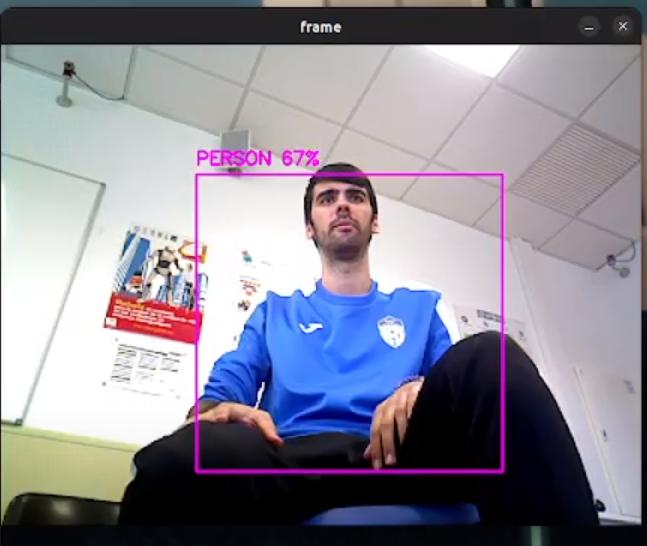
\includegraphics[width=7cm]{figs/c5/sec_rot1.png}
        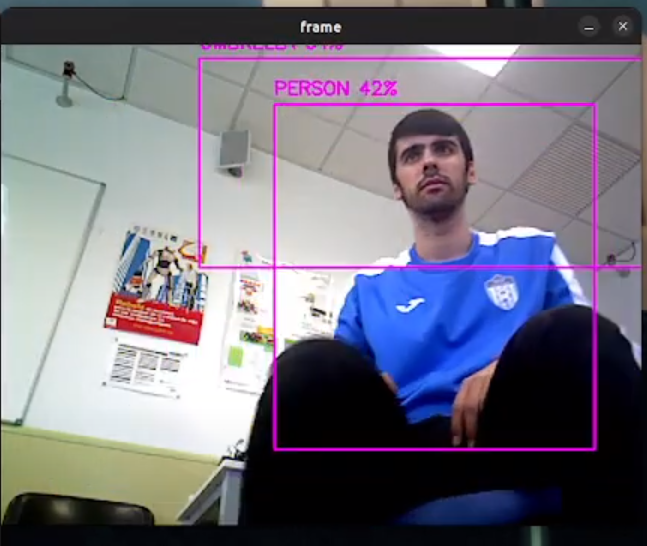
\includegraphics[width=7cm]{figs/c5/sec_rot2.png}
        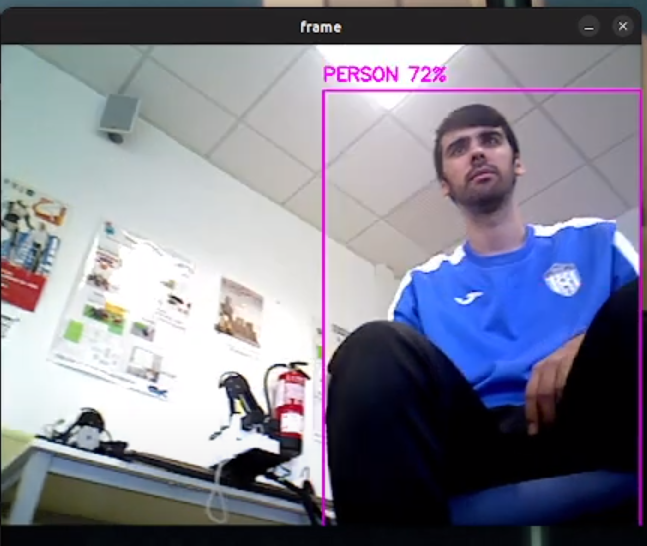
\includegraphics[width=7cm]{figs/c5/sec_rot3.png}
        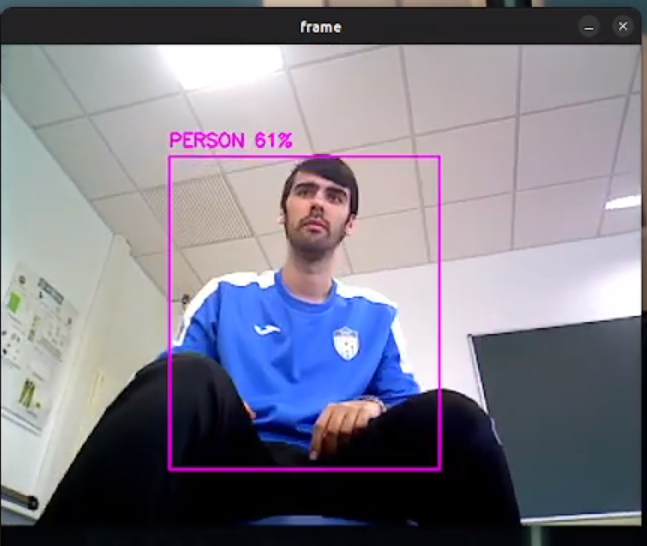
\includegraphics[width=7cm]{figs/c5/sec_rot4.png}
    \end{center}
    \caption[Secuencia sigue-personas rotación]{Secuencia de imágenes del sigue-personas. Imagenes obtenidas de Youtube\footnotemark.}
    \label{fig:sec_FP_rot}
\end{figure}
\footnotetext{\textbf{Vídeo}: \url{https://www.youtube.com/watch?v=Uir_iqMOplc&ab_channel=Tapii}}

\section{Modificaciones al sigue-personas para incluir movimiento lineal.}
\label{sec:FP_2}

Para añadir el comportamiento de seguir linealmente a la persona, debemos leer también la información sobre la profundidad que nos da la cámara.
Para ello vamos a crear un bloque usando el modelo de bloques de sensores que usamos anteriormente (\ref{sec:drivers_creacion}).
También cambiaremos el funcionamiento general de varios bloques para optimizar y reducir el número de \textit{inputs} y bloques del circuito.

\begin{figure} [H]
    \begin{center}
        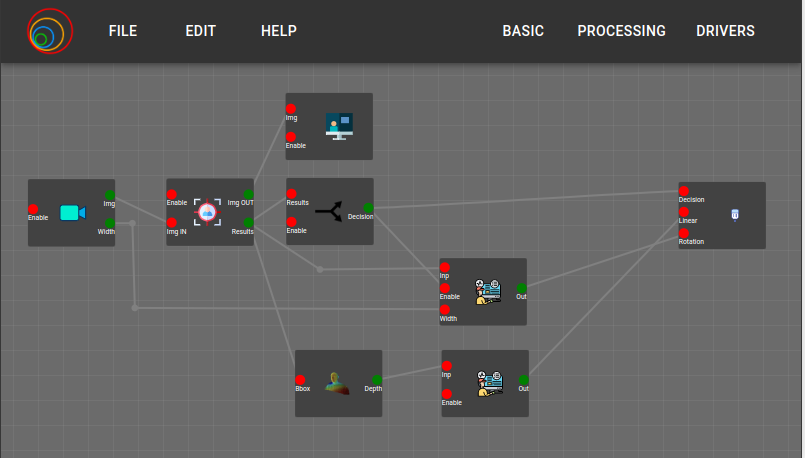
\includegraphics[width=12cm]{figs/c5/follow_person_final_model.png}
    \end{center}
    \caption[Circuito sigue-personas inicial]{Circuito inicial del algoritmo sigue-persona.}
    \label{fig:final_follow_person}
\end{figure}

Como podemos ver, toda la rama inferior de bloques es la que se encarga del movimiento lineal, mientras que la superior se encarga del movimiento angular.
La única parte de la parte superior que ha cambiado es que ya no existe un bloque que envíe siempre la velocidad de rotación, en cambio está directamente en el
bloque que envía la velocidad a los motores y, dependiendo de la decisión, se envía la rotación estática o se envían las velocidades de los bloques PID.

\begin{code}[H]
    \begin{lstlisting}[language=python]
        while auto_enable:
            try:
                decision = inputs.read_number("Decision")
                if(decision == 0):
                    velocities = [0,0,0,0,0,0.05]
                else:
                    velocities = inputs.read_array('Vels2')
                    velocities[0] = inputs.read_number('Linear')
            except Exception:
                continue

    \end{lstlisting}
    \caption[Código bloque MotorDriver sigue-persona modificado]{Código del bloque del \textit{MotorDriver} sigue-persona modificado.}
    \label{cod:MotorDriver_FP_final}
\end{code}

\begin{figure} [H]
    \begin{center}
        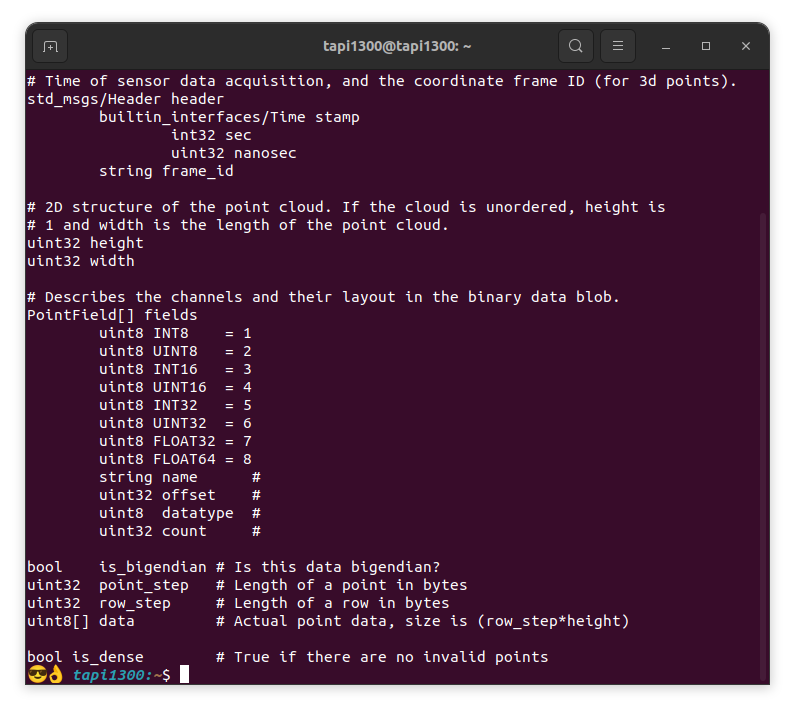
\includegraphics[width=10cm]{figs/c5/PointCloud2_data.png}
    \end{center}
    \caption[Estructura mensaje PointCloud2]{Estructura del tipo de mensaje \textit{sensor\_msgs/msg/PointCloud2.}}
    \label{fig:PC2_struct}
\end{figure}


En cuanto a la rama inferior, el bloque principal es el que recibe la información de la profundidad. Esta información viene en forma
de \textit{PointCloud2} (\textit{sensor\_msgs/msg/PointCloud2}) que, como  podemos ver en la imagen \ref{fig:PC2_struct}, envía los datos del sensor en el
campo \textit{data}, por lo que esto será lo que guardemos en la variable global del bloque del sensor y será lo que enviemos por el cable.\\

La forma en la que se guardan los datos dentro de este campo es en bytes y es la siguiente para cada punto de la cámara (640x480 = 307200 puntos):
12 bytes para x,y,z (4 bytes cada coordenada), 4 bytes vacíos, 4 bytes para el color del punto y otros 12 bytes vacíos. Esto hace que en el \textit{array} de datos
nos aparezcan 9830400 valores y la búsqueda final sea el número de filas (coordenada Y) por el ancho total de la imagen más la posición actual de nuestra coordenada X
multiplicado por 32 (posiciones que ocupa cada pixel en el array) y sumamos 8 para obtener la posición inicial de la coordenada Z. Luego, usando la función
``\textit{unpack}" del paquete \textit{struct} podemos transformar los siguiente 4 bytes (correspondientes a la coordenada Z) en un \textit{float} y obtener
la distancia entre el robot y el centro de la \textit{BoundingBox} de la persona.

\begin{code}[H]
    \begin{lstlisting}[language=python]
    # IMPORT
    from sensor_msgs.msg import PointCloud2
    from struct import unpack

    # CALLBACK DENTRO DE LA CLASE
        def callback(self, msg):
            global measure
            measure = msg.data

    # BUCLE DENTRO DEL MAIN
        while(1):
            bbox = inputs.read_array("Bbox")
            if bbox is None:
                continue
            try:
                x = int(bbox[0]+bbox[2]/2)
                y = int(bbox[1]+bbox[3]/2)
            except:
                continue

            rclpy.spin_once(depth_subscriber)
            point = (width*y+x)*32+8
            depth = unpack('f', measure[point:point+4])
            outputs.share_array("Depth",depth)   
            synchronise()
    \end{lstlisting}
    \caption[Código bloque Camera-Depth sigue-persona]{Código del bloque del \textit{PointCloud2} del sigue-persona.}
    \label{cod:PC2_block_FP}
\end{code}

Esta información llega a un segundo bloque PID, que es el que se va a encargar de mantener esta distancia con la persona en 1.5 metros. El código de este bloque
es similar al del otro bloque PID (\ref{cod:PID_follow_person}), pero ahora no necesitamos una velocidad límite (el mínimo y máximo que conseguiremos no es peligroso
en comparación a las velocidades angulares altas).

\begin{code}[H]
    \begin{lstlisting}[language=python]
        import numpy as np
        import math
        from time import sleep
        
        def main(inputs, outputs, parameters, synchronise):
            auto_enable = True
            try:
                enable = inputs.read_number("Enable")
            except Exception:
                auto_enable = True
            kp = parameters.read_number("Kp")
            ki = parameters.read_number("Ki")
            kd = parameters.read_number("Kd")
            previousError, I = 0, 0
            while(auto_enable or inputs.read_number('Enable')):
                msg = inputs.read_number("Inp")
                if msg is None:
                    continue
                error = float(msg) - 1.5
                sleep(0.01)
        
                P = error
                D = error - previousError
                PIDvalue = (kp*P) + (kd*D)
                previousError = error
    
                linear_velocity = PIDvalue
                if msg == 0:
                    linear_velocity = 0
                outputs.share_number("Out", linear_velocity)
                synchronise()
    \end{lstlisting}
    \caption[Código bloque PID lineal sigue-persona]{Código del bloque del PID de velocidad lineal del sigue-persona.}
    \label{cod:PID_linear_FP}
\end{code}

\section{Pruebas en el robot real y resultado final.}
\label{sec:FP_final}

Ahora que ya está configurado el comportamiento correctamente, tanto la velocidad lineal para mantenerse a 1.5 metros como la velocidad angular para
mantener al humano en el centro de la visión del robot, es hora de probarlo en el robot real.\\

Para configurar correctamente los sensores del robot real debemos tener instalados los paquetes referentes a lanzar el kobuki (\ref{subsec:turtlebot2_base}),
al igual que los necesarios para usar la cámara (\ref{subsec:asus_xtion}).
De aquí usaremos los siguientes comandos para conseguir que todo funcione correctamente:

\begin{code}[H]
    \begin{lstlisting}[language=bash]

$> ros2 launch asus_xtion asus_xtion.launch.py

$> ros2 launch ir_kobuki kobuki_rplidar.launch.py
    \end{lstlisting}
    \caption[Comandos para lanzar kobuki y cámara]{Comandos para activar la cámara con ROS2 y lanzar el kobuki con el láser.}
    \label{cod:coms_kobuki_laser_cam}
\end{code}

Una vez probado, podemos comprobar los resultados mirando el vídeo en el que se explica el funcionamiento de los bloques (como ya se ha explicado en las
secciones \ref{sec:FP_intro} y \ref{sec:FP_2}) y se muestra un ejemplo de ejecución con el robot real en los laboratorios:


\begin{figure} [H]
    \begin{center}
        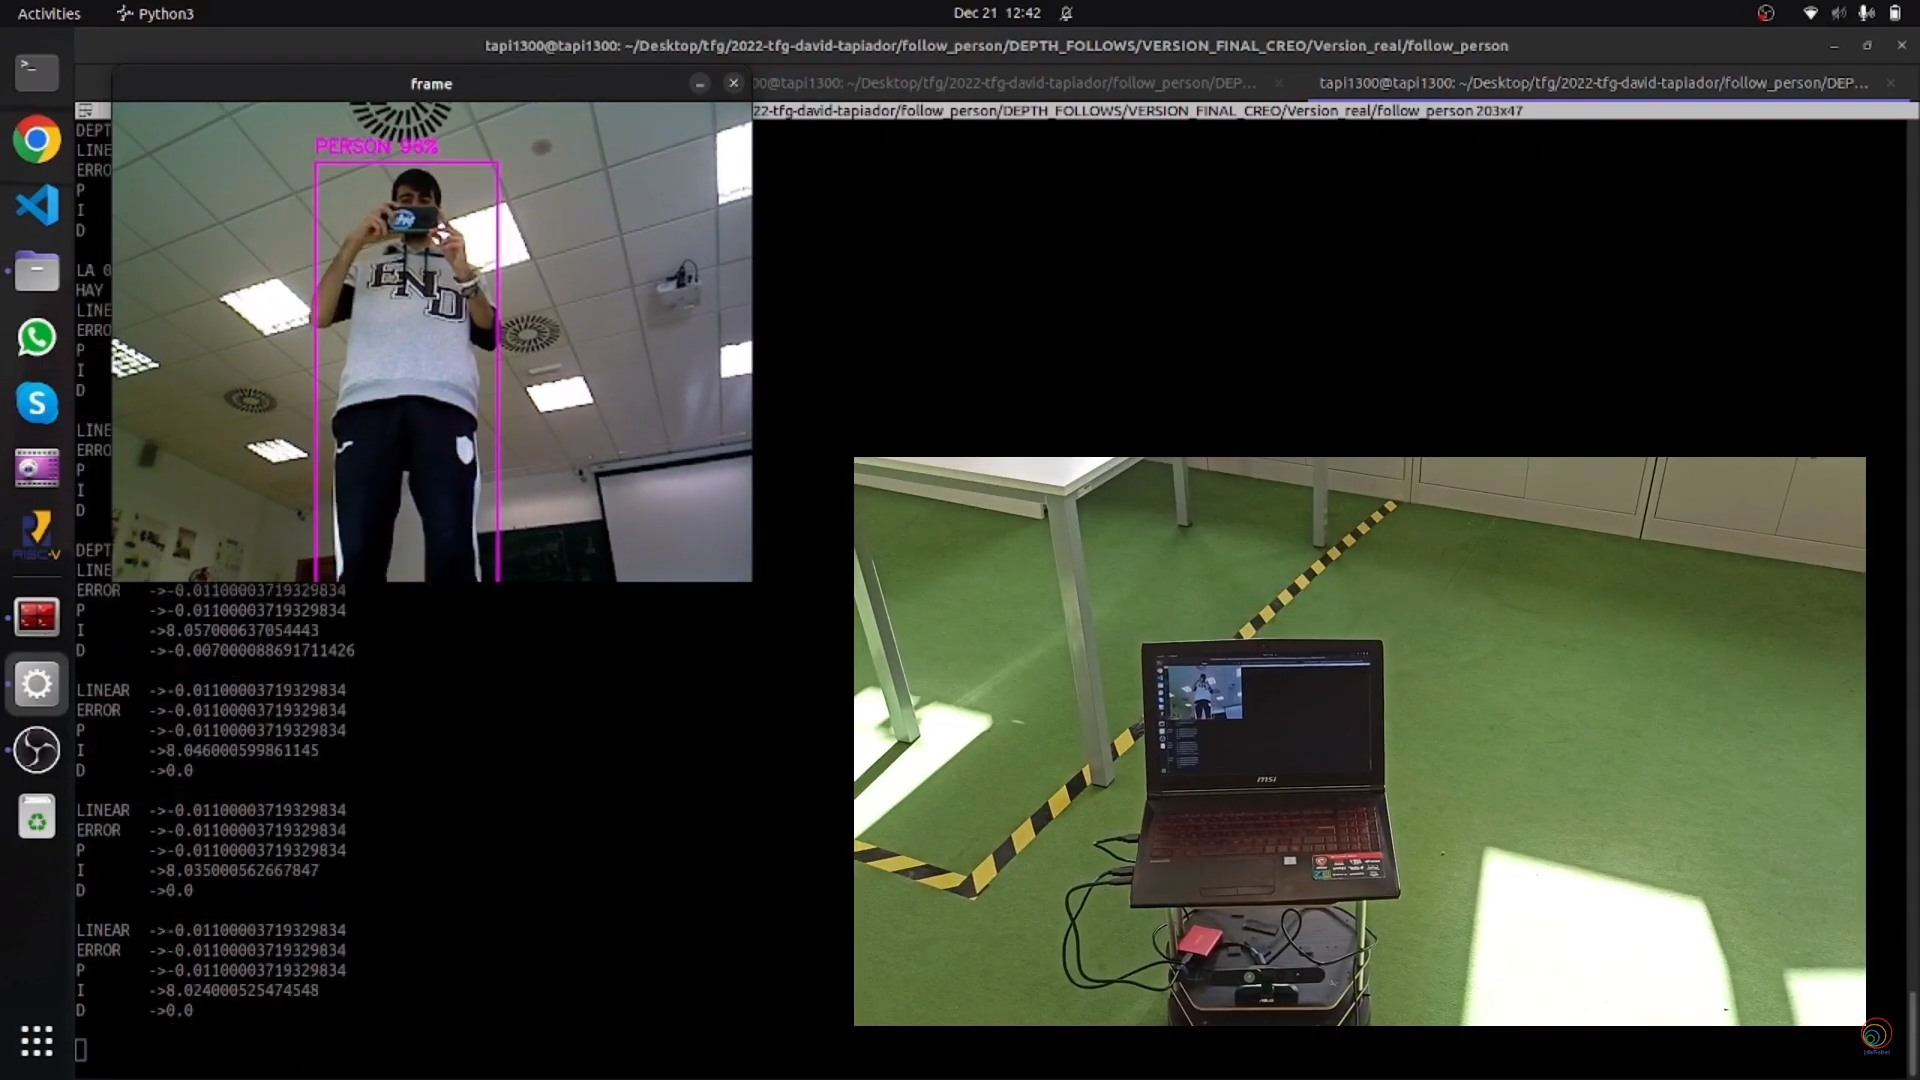
\includegraphics[width=7cm]{figs/c5/fp_final1.png}
        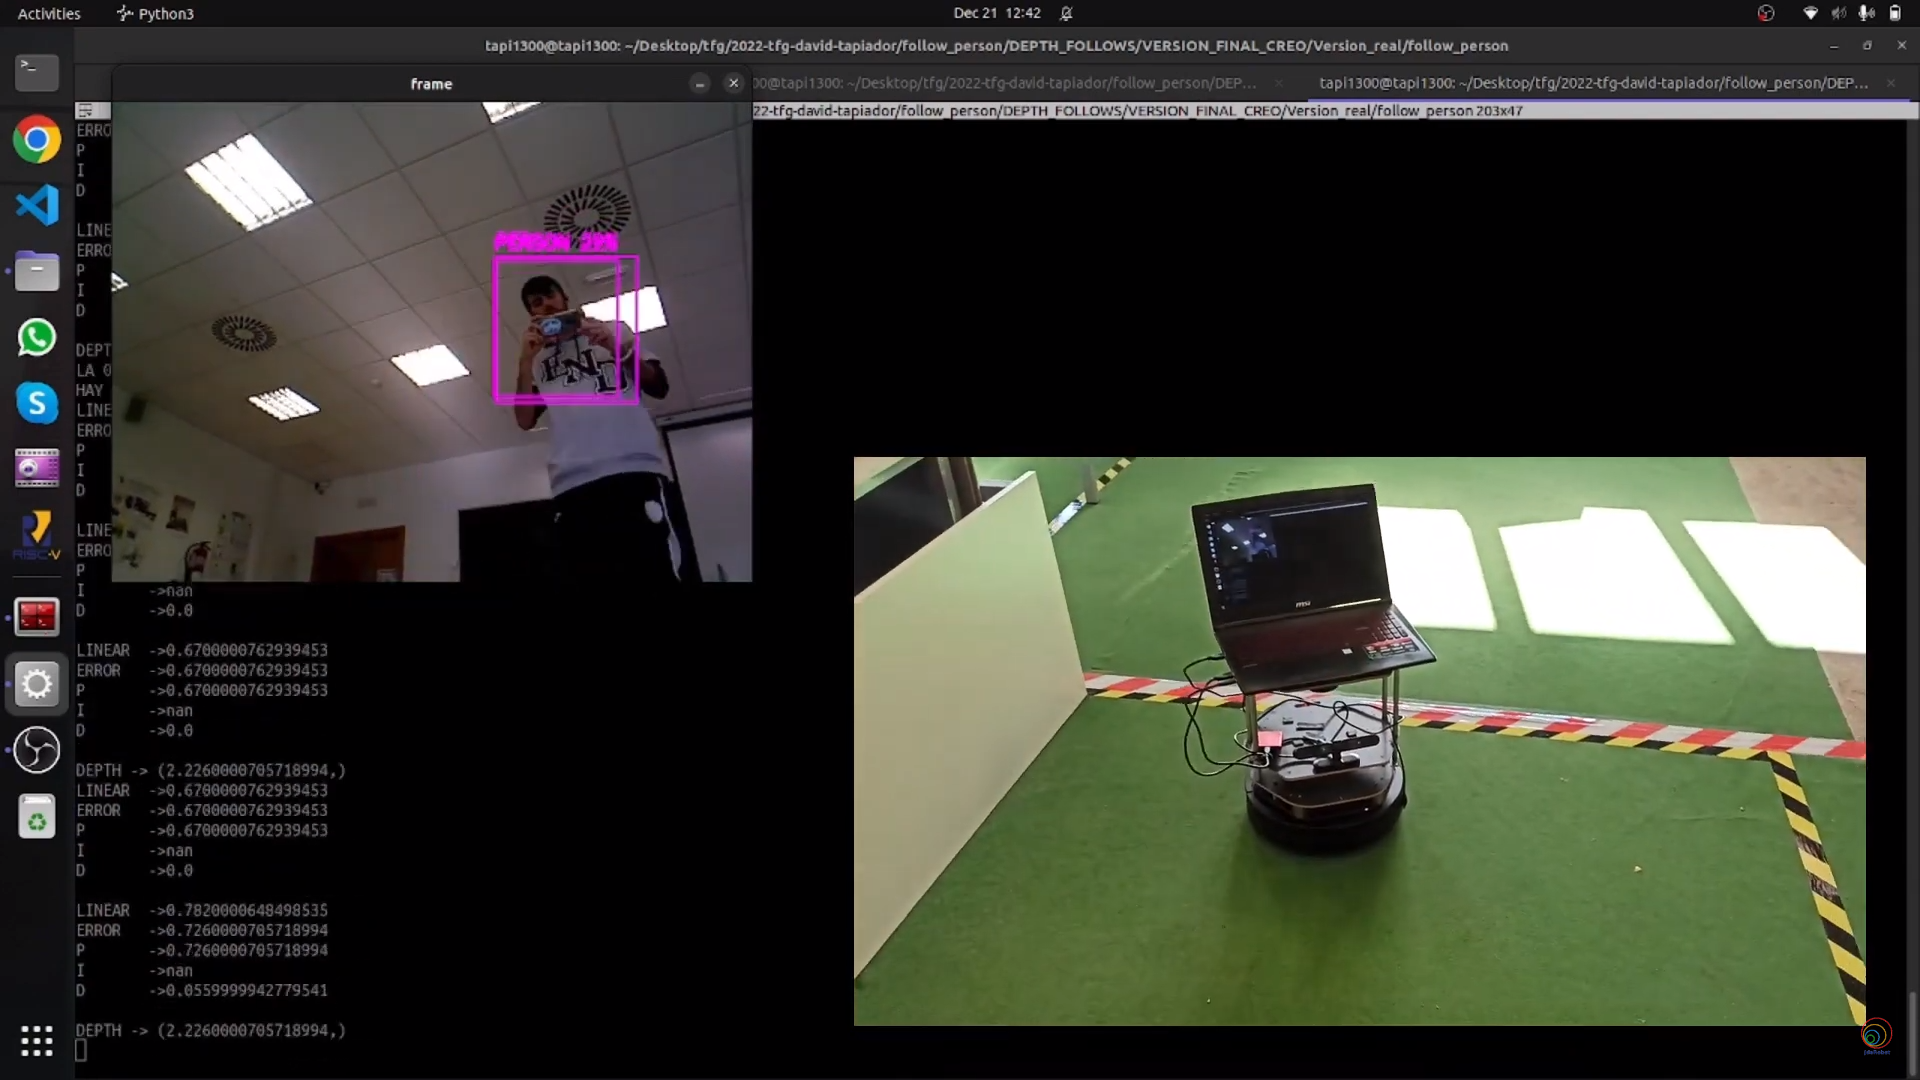
\includegraphics[width=7cm]{figs/c5/fp_final2.png}
        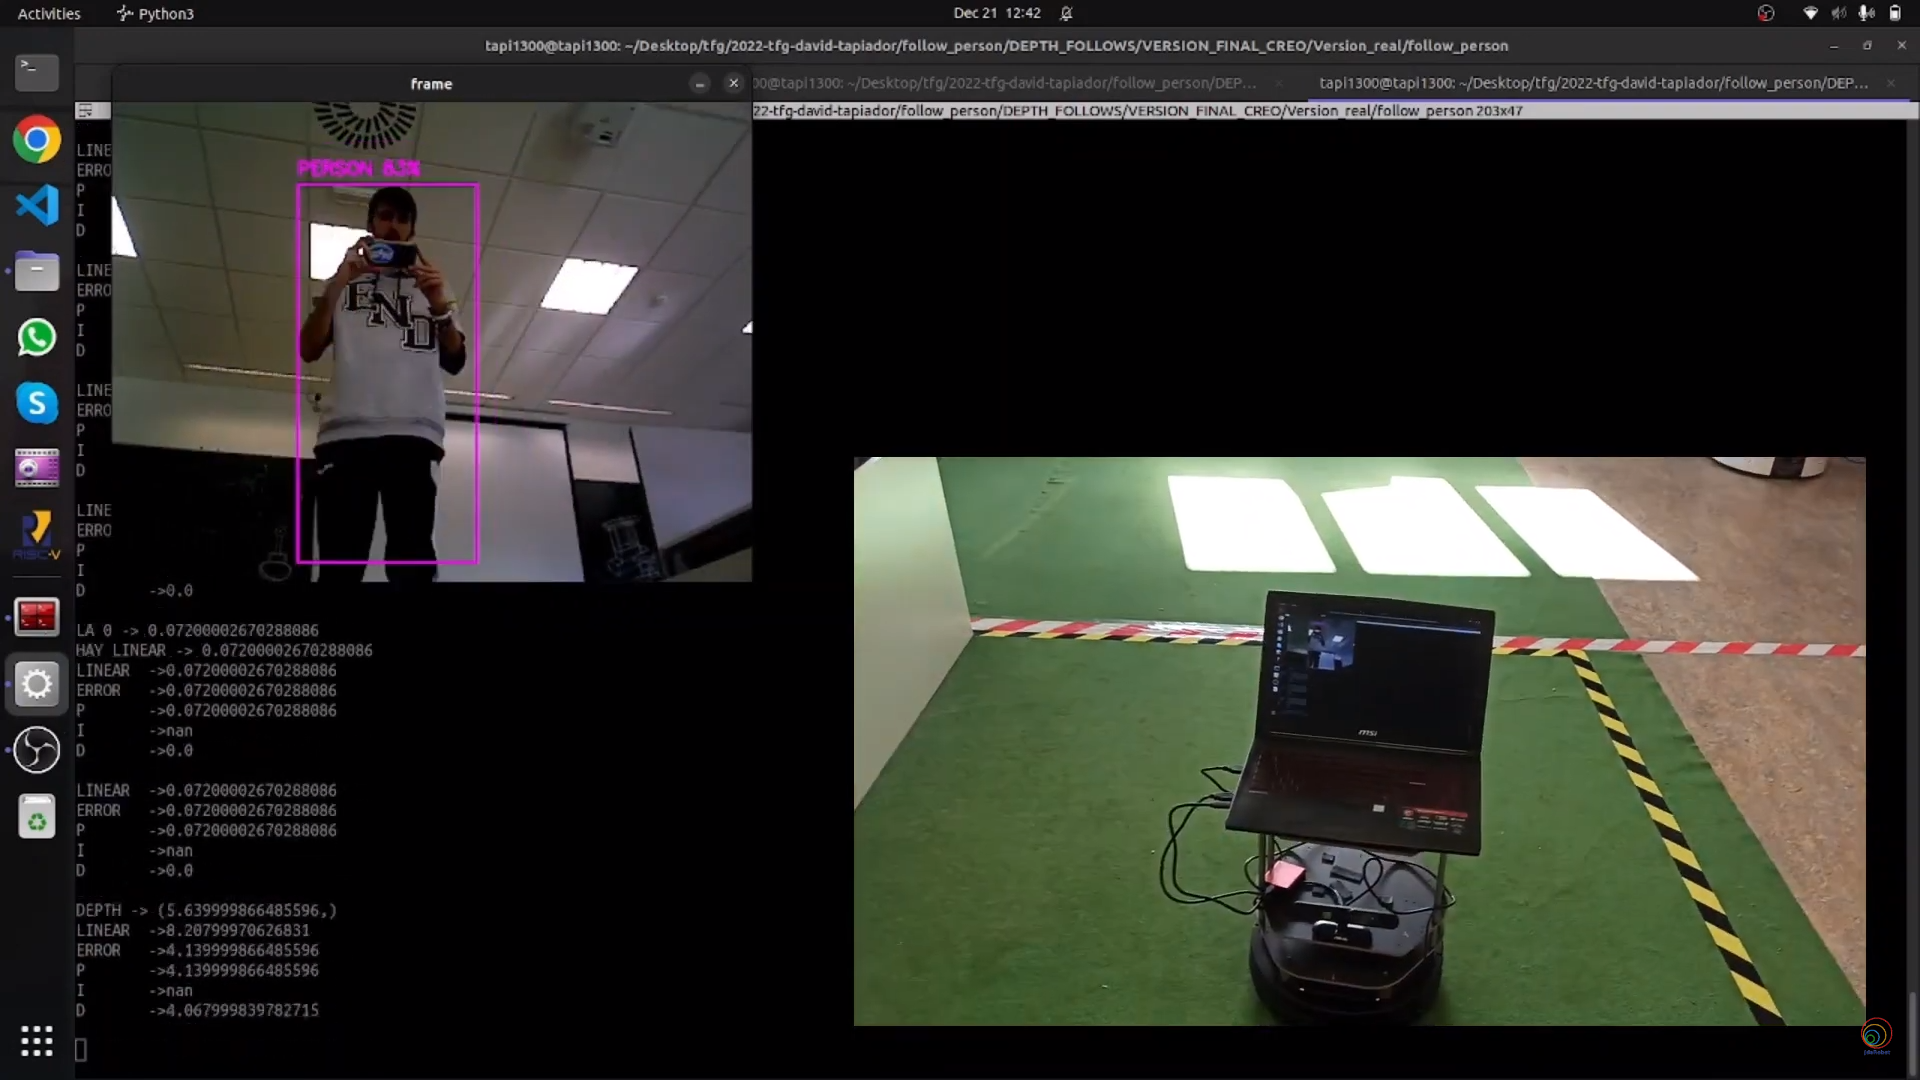
\includegraphics[width=7cm]{figs/c5/fp_final3.png}
        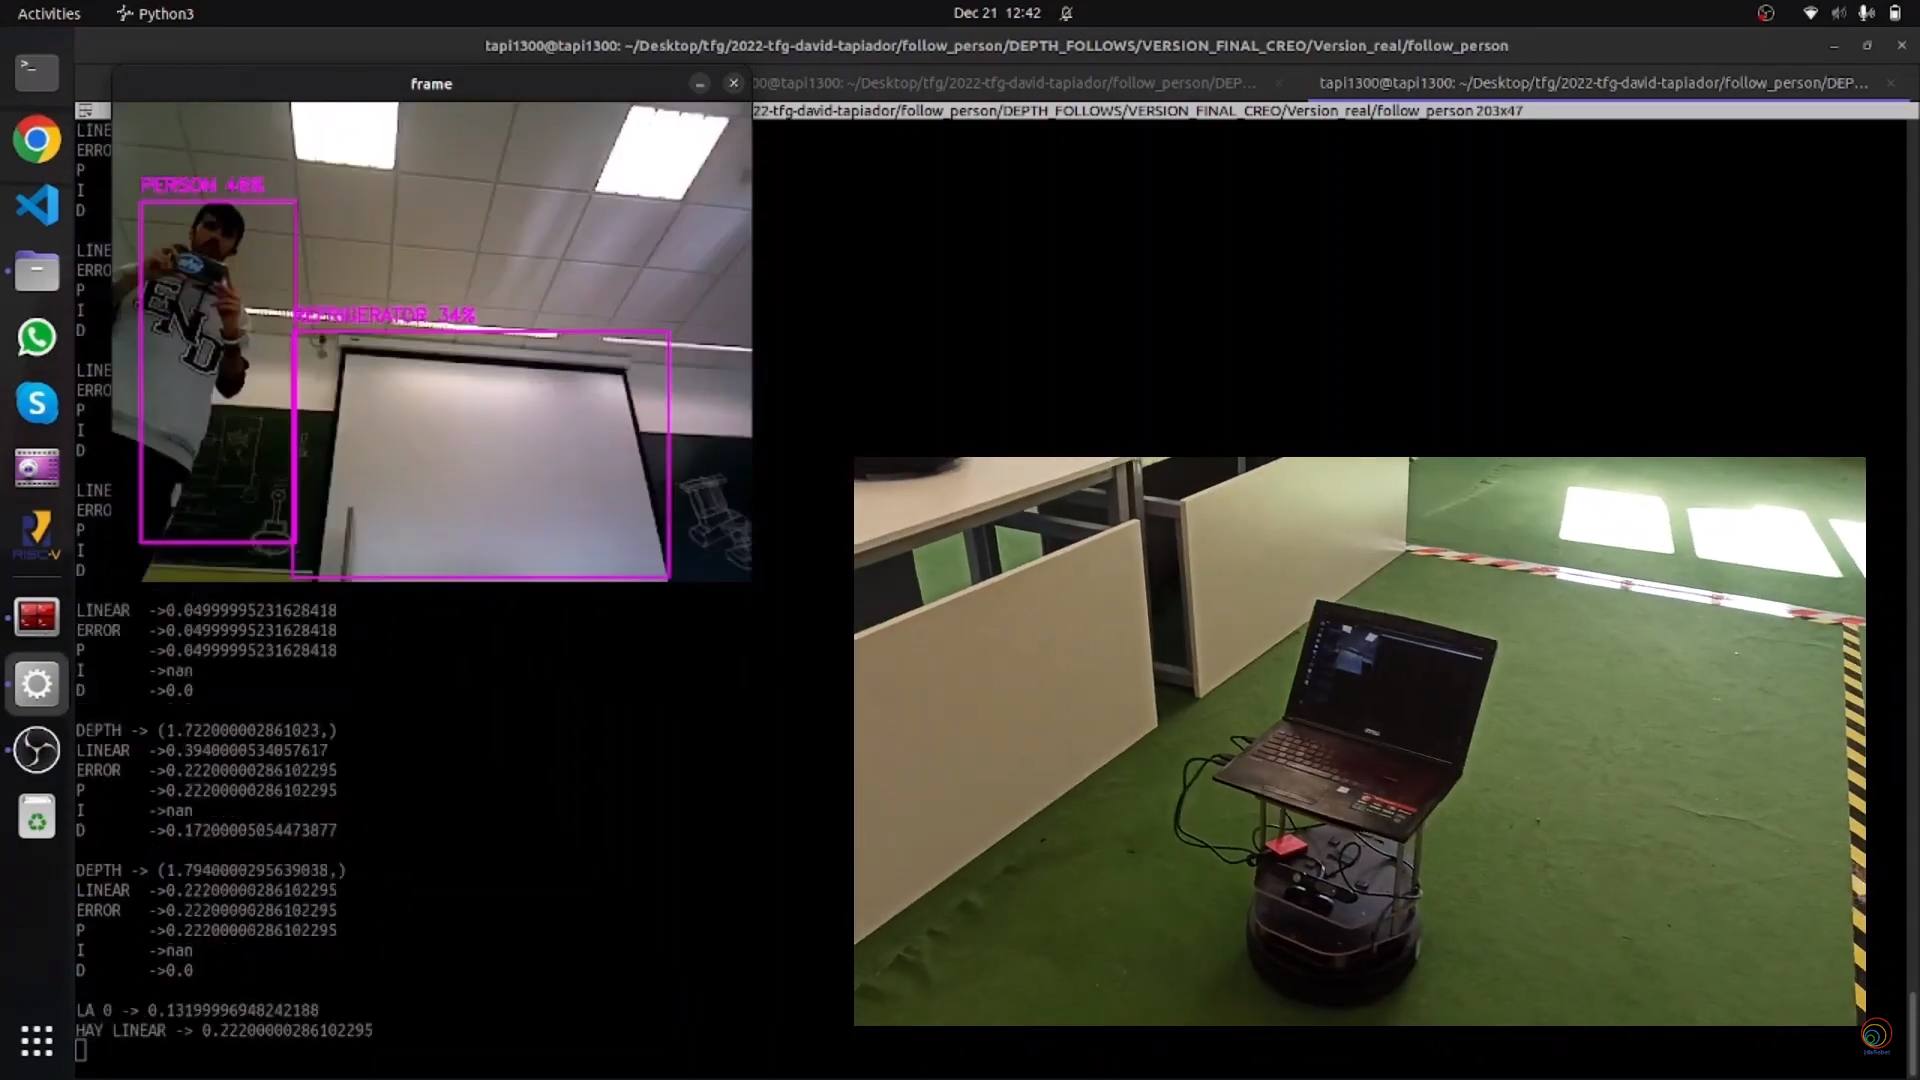
\includegraphics[width=7cm]{figs/c5/fp_final4.png}
    \end{center}
    \caption[Secuencia sigue-personas resultado final]{Secuencia de imágenes del sigue-personas. Imagenes obtenidas de Youtube\footnotemark.}
    \label{fig:sec_FP_final}
\end{figure}
\footnotetext{\textbf{Vídeo}: \url{https://www.youtube.com/watch?v=IknpvAs_jAo&ab_channel=JdeRobot}}

































































